% Author : Prakash Gautam
% Date   : 19-07-2020 00:10:58
%
\documentclass[a4paper]{article}

\usepackage{amsmath}
\usepackage{amssymb}
\usepackage{physics}
\usepackage{graphicx}
\usepackage{tikz}
%\usepackage{tikz-feynman}
\usepackage{pgf}
\usepackage{pgfplots}
%\usetikzlibrary{axis}
\usetikzlibrary{
    backgrounds,
    calc,
    decorations.fractals,
    decorations.pathmorphing,
    decorations.pathreplacing,
    decorations.shapes,
    decorations.text,
    decorations.markings,
    fit,
    math,
    matrix,
    mindmap,
    positioning,
    quotes,
    shapes
}
%\usetikzlibrary{decorations.markings,decorations.pathreplacing,arrows.meta,calligraphy,calc,math}

\author{Prakash Gautam}
\title{Practicing Ti{\em kZ} diagrams.}

%\pgfplotsset{compat=1.16}
\begin{document}
    \maketitle
    \section{Introduction}
        We have some text and we have Kapindra in the house.
        \begin{figure}[h!]
            \centering
            %\begin{tikzpicture}
    \node [anchor=west] (note) at (-1,3) {Curvature Note};
    \node [anchor=west] (water) at (-1,1) {First Bump};
    \begin{scope}[xshift=1.5cm]
        \node[anchor=south west,inner sep=0] (image) at (0,0) {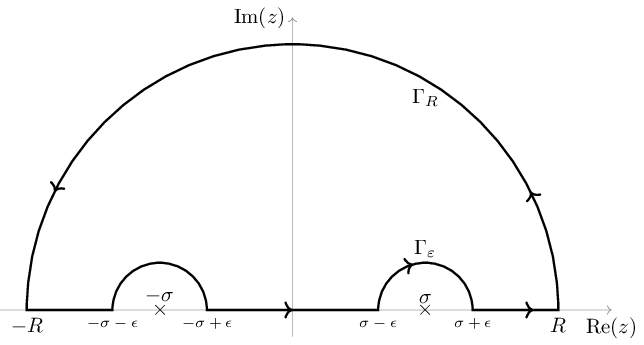
\includegraphics[width=0.7\textwidth]{../tikz/complex_integration_2.png}};
        \begin{scope}[x={(image.south east)},y={(image.north west)}]
            \draw[red,ultra thick,rounded corners] (0.48,0.80) rectangle (0.55,0.95);
            \draw [-latex, thick, red] (note) to[out=0, in=-120] (0.48,0.80);
            \draw [-stealth, line width=1pt, cyan] (water) -- ++(0.37,0.0);
        \end{scope}
    \end{scope}
\end{tikzpicture}%

            %\usetikzlibrary{arrows.meta,shapes.multipart}
\begin{tikzpicture}[
  thick,>={Stealth[]},
  ampersand replacement=\&,
  circ/.style = {draw,circle,minimum size=1cm},
  rect/.style = {draw,rectangle,minimum size=1cm},
  splt/.style = {draw,rectangle split,rectangle split parts=5,minimum size=0.5cm}
  ]
  \matrix[row sep=1cm,column sep=1cm] {
     {}; \&
     \node[rect] (Tr) {Train Dataset};  \&
     \node[rect] (A) {ML Algorithm}; \&
     {};\\

     \node[splt, minimum size=25mm] (D) {Dataset}; \&
     {};\&
     \node[rect, minimum size=15mm] (M) {Model}; \&
     \node[circ] (V) {Validate};\\

     {};\&
     \node[rect] (Te) {Test Dataset};
     {}; \&
     {}; \&\\
  };
  \draw[->] (D)  --(Tr);
  \draw[->] (D) --(Te);
  \draw[->] (Tr) --(A);
  \draw[->] (Te) --(M);
  \draw[->] (A) --(M);
  \draw[->] (M) --(V);
\end{tikzpicture}

            \input{/home/pranphy/.Rough/python/images/SineCurve.tex}
            \caption{Name}
            \label{fig:name}
        \end{figure}
    \section{Inline tikz}
    Is this inline \tikz \draw[color=red,fill] (0,0) circle (4pt); and we continue this and we continue this. And a rectangle \tikz \draw[fill,color=black] (0,0) rectangle (.2,.2); is here
\end{document}
